\documentclass{article}

% Language setting
% Replace `english' with e.g. `spanish' to change the document language
\usepackage[english]{babel}
\usepackage{tabularx}
\usepackage{subfigure}
\usepackage{amsmath}

% Set page size and margins
% Replace `letterpaper' with `a4paper' for UK/EU standard size
\usepackage[letterpaper,top=2cm,bottom=2cm,left=3cm,right=3cm,marginparwidth=1.75cm]{geometry}

% Useful packages
\usepackage{amsmath}
\usepackage{graphicx}
\usepackage[colorlinks=true, allcolors=blue]{hyperref}

\title{Control Policy Design for Path Planning and Obstacle Avoidance Using Adpative Model Predictive Control of a Four-Wheel Based Extraterrestrial Rover}
\author{Jason Zhou\{zzhou292@wisc.edu\}, Yulong Yue\{yyue32@wisc.edu\}}

\begin{document}
\maketitle


\section{Research Problem Statement}
In this project, we proposed to design a rover path planning and following algorithm to provide an extraterrestrial rover navigation strategy. We propose to solve the problem by solving a closed-loop motion planning and control problem based on optimization with constraints. The control strategy will be benched in a simulated environment in Project Chrono. For the project, we will assume privileged information, such as locations, sizes, and shapes of the obstacles. Also, we will assume the environment is limited and fixed. 


\section{Background}
\subsection{Rover Control Strategy}
Providing control solutions to extraterrestrial rover can always be challenging, due to the low tolerance to mistake and long signal transmission delay. Nowadays, most space exploration agencies, such as The National Aeronautics and Space Administration (NASA), are adopting two different ways for rover control:

\begin{itemize}
    \item Manual Explicit Motion Commands
    \item A propitiatory Autonomous Path Planning and Path Following Control Policies
\end{itemize}

The first manual control strategy is relatively simple. Based on the images transmitted from the rover, the ground base provides direct motion commands, such as "move forward for 5m", to the rover. The method relies heavily on human judgment, along with data and command transmission, which usually suffer from the signal delay between the ground base on earth and extra extraterrestrial planets. This control method will not be discussed in the project.

The second control method, although proprietary and few details have been disclosed by NASA, is an autonomous path planning and trajectory following control algorithm which matches the materials covered in the class. Based on the introduction provided by NASA, the ground base on earth, based on the images and data transmitted from the rover, sends a control signal containing the location of the next 'waypoint'. Then the rover, based on its own sensing capabilities using sensors such as camera and lidar, plans the route and tracking the planned trajectory. \cite{NASAweb}

\subsection{Simulation Through Project Chrono}
Project Chrono is a multi-physics modeling and simulation infrastructure based on a platform-independent, open-source design. Project Chrono has been used widely for the simulation of autonomous vehicles and robotic systems. Project Chrono, in the past two years, received funding from NASA to provide simulation support to investigate wheel-terrain interaction of the 2024 NASA VIPER Moon Rover using different types of terra-mechanics simulation method, as shown in Figure \ref{fig:viper_chrono} and Figure \ref{fig:curiosity_chrono}. Therefore, the software package already contains multiple ready-to-deploy extraterrestrial rover models and their control interfaces. 

In this project, we will develop the algorithm in Matlab, and use Project Chrono as our simulation environment. In the simulation, we will use the Soil-Contact Model (SCM) deformable terrain model to simulation soil deformation. The SCM model is a simple semi-empirical model which is built upon the original Bekker-Wong Equation, as shown in Equation \ref{equ:bekker}. A more detailed description can be found in \cite{10.1115/1.4056851}. In the Equation \ref{equ:bekker}, \(K_{c}\), \(K_{\phi}\), and n are semi-empirical parameters defining the soil properties, \(z\) is the sinkage, \(b\) is the average wheel contact width, and \(p\) is the normal pressure applied to the rover wheel (to provide normal force in the simulation).

\begin{equation}\label{equ:bekker}
	p = \left( \frac{K_c}{b} + K_\phi \right) z^n \, .
\end{equation}

\begin{figure}
	\centering     %%% not \center
	\subfigure[Curiosiy Mars rover on SCM deformable terrain with lidar and radar sensing simulation]{
		\label{fig:curiosity_chrono}
		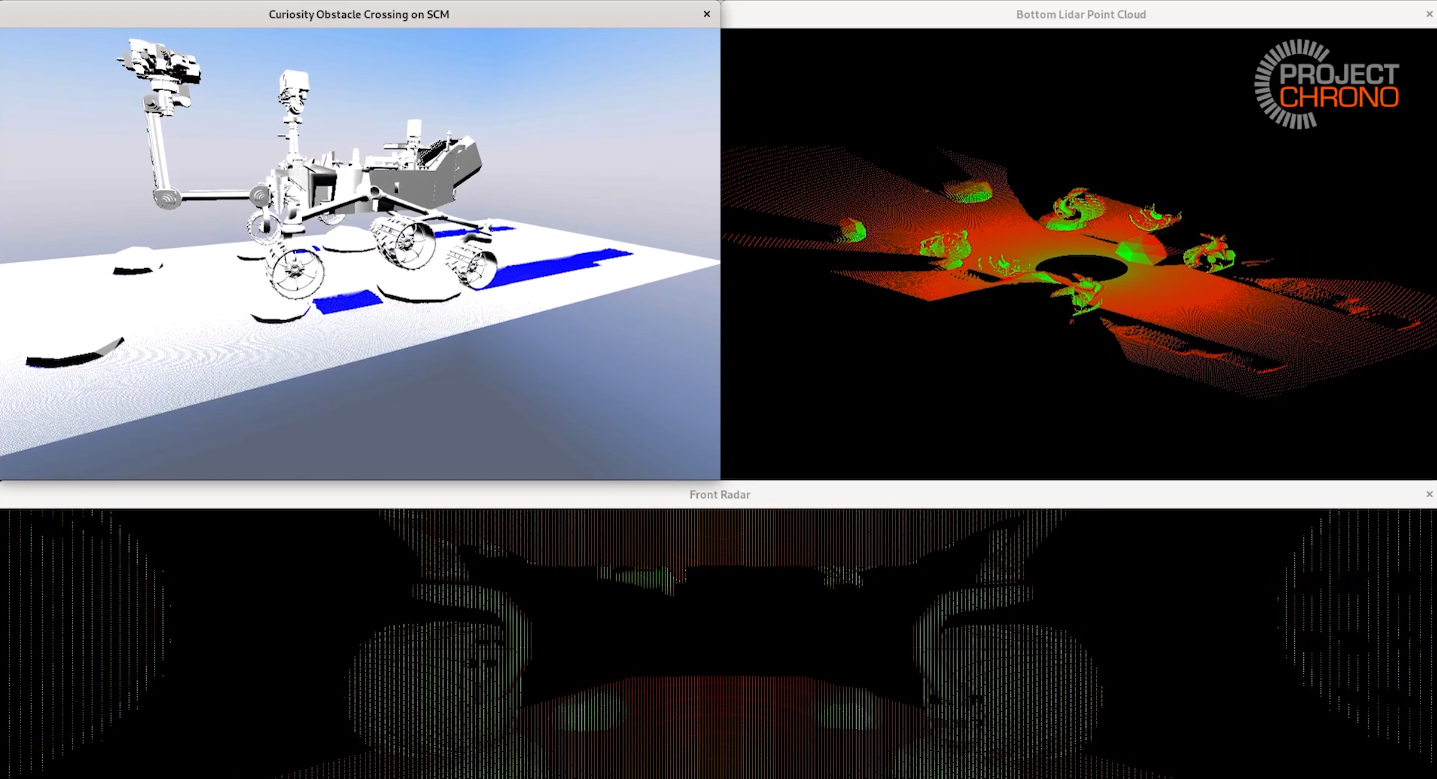
\includegraphics[width=0.45\textwidth]{Images/Curiosity_Sensing.png}}
	\subfigure[VIPER Lunar rover conducting bulldozing experiment on granular terrain simulated by Smoothed-Particle Hydrodynamics (SPH) Method]{
		\label{fig:viper_chrono}
		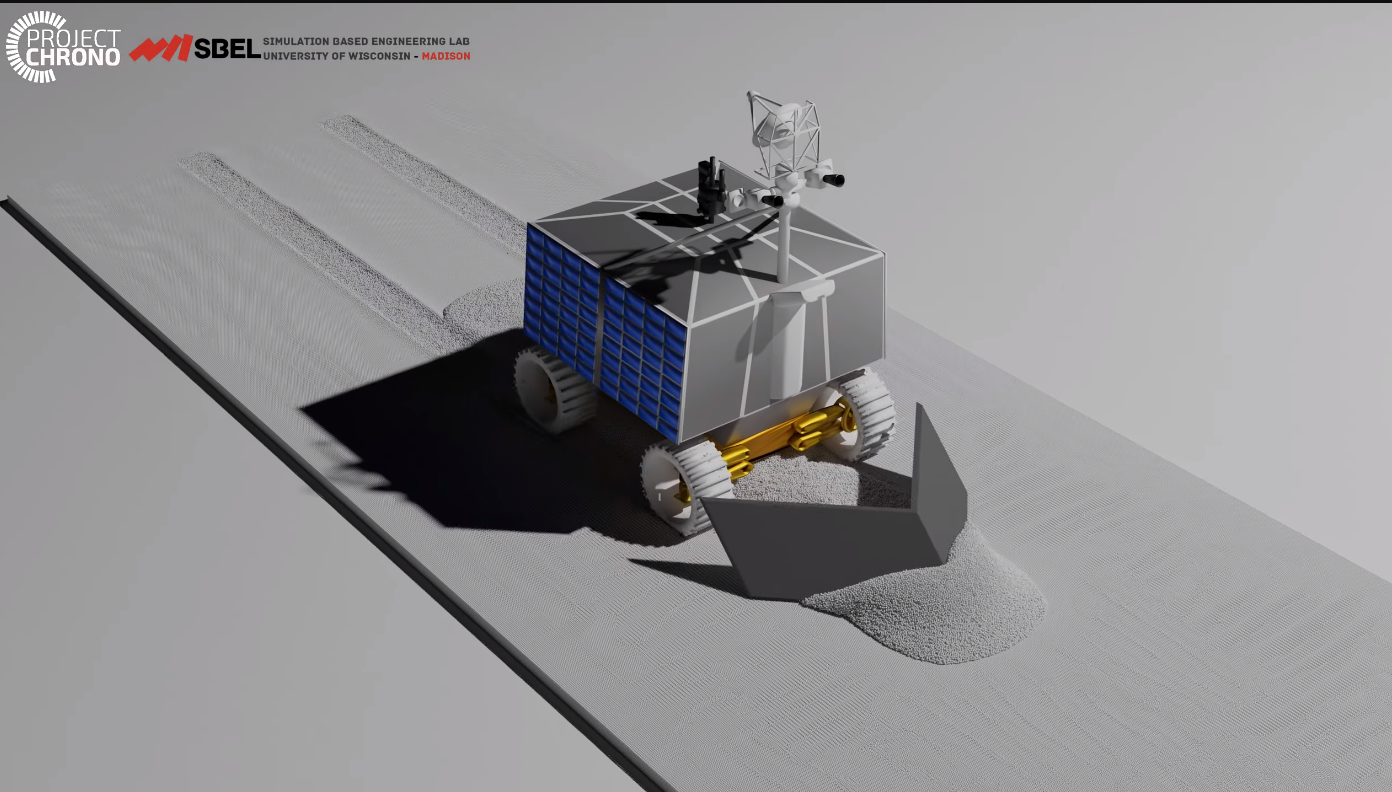
\includegraphics[width=0.45\textwidth]{Images/Viper_Bull.png}}
	\caption{Project Chrono contains complete rover models, control interfaces, and deformable terrain models for wheel-terrain interaction}
\end{figure}


\section{Proposed Solution}

The problem will be simplified into an optimal path planning and control optimization problem by assuming a square terrain with a center at (0.0, 0.0), and a fixed side length a. We will use two different types of rocks with different sizes as our obstacle. To further simplify the problem, a bounding circle, or what can be called a safety circle, will be drawn around the rock. From a bird's eye view, looking from above, the problem environment will be simplified into a 2D path planning and optimal control problem with a given square terrain, and with several rectangular-shaped obstacles, as shown in Figure \ref{fig:rover_path}.

We employ car model as shown in Equations \ref{equ:car_dyn}.

\begin{equation}
\label{equ:car_dyn}
  \left\{\begin{array}{@{}l@{}}
    \dot{x}=vcos\theta  \\
    \dot{y}=vsin\theta  \\
    \dot{\theta} = \frac{v}{L}tan\phi \\
  \end{array}\right.\,.
\end{equation}

After the simplification, we assume that each obstacle has the properties shown in Equation \ref{equ:opt}, in which \(x_{obs_{k}}\) and \(y_{obs_{k}}\) represent the location of the k'th obstacle's bounding circle, and \(r_{obs_{k}}\) represent the radius of the bounding circle of the k'th obstacle. If we assume the entire time domain of the problem contains N steps, and there are M obstacles presented in the environment, the optimization control can be expressed and modelled as shown in Equations \ref{equ:opt}. Assuming the starting location of the rover is \([\) \(X_{start}\), \(Y_{start}\) \(]\), and the given target location is \([\) \(X_{end}\), \(Y_{end}\) \(]\). We use control effort as our cost function and assume minimum control effort as our optimization strategy.

\begin{equation}
\label{equ:opt}
\begin{aligned}
\min_{w,b,\xi} \quad & \sum_{i=0}^{N}{u_{i}^2}\\
\textrm{s.t.} \quad & x_{N} = x_{end}, y_{N} = y_{end} \\
    & x_{0} = x_{start}, y_{N} = y_{start} \\
    &    \dot{x}=vcos\theta  \\
    & \dot{y}=vsin\theta  \\
    & \dot{\theta} = \frac{v}{L}tan\phi \\
  &x_{i} < x_{obs_{k}}-r_{obs_{k}}, y_{i} < y_{obs_{k}}-r_{obs_{k}}    \\
  &x_{i} > x_{obs_{k}}+r_{obs_{k}}, y_{i} > y_{obs_{k}}+r_{obs_{k}}   \\
  & 0 \leq i \leq N, 0 \leq k \leq M \\
\end{aligned}
\end{equation}
 

\begin{figure}
\centering
    \label{fig:rover_path}
    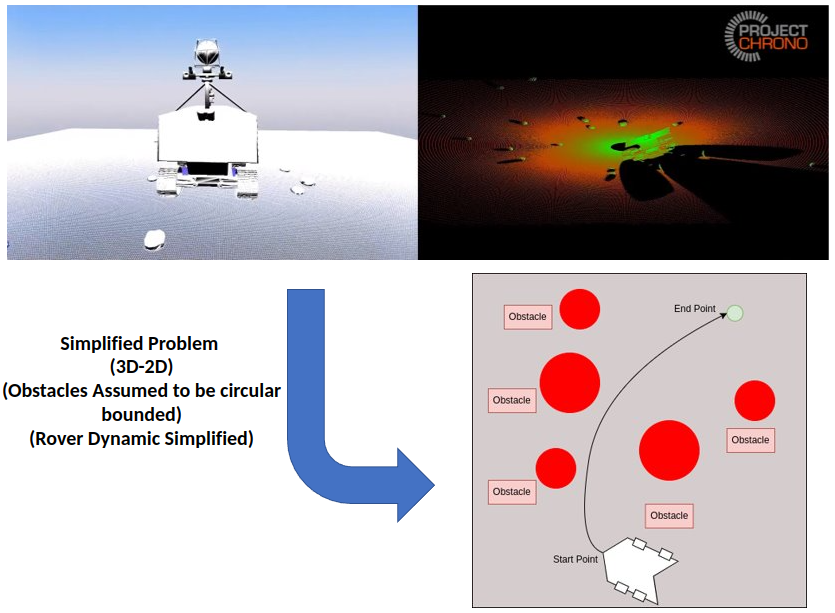
\includegraphics[width=0.85\textwidth]{Images/rover_path.png}
    \caption{The problem will be simplified into a 2-dimensional path planning and optimal control problem. The optimization will be solved in the 2-D space and applied and benched in the 3-D simulation.}
\end{figure}

After the optimization problem has been solved, a control input series \(u_{opt}\) and a control path series defined by \(x_{opt}\) and \(y{opt}\) are expected to be the output. However, the control input series \(u_{opt}\) will need to be post-processed in order to feed into the Chrono simulation. This is due to the fact that the simplified rover dynamic equations defined in Equation \ref{equ:car_dyn} is a significantly simplified control, by inputting steering angle and rover velocity. However, the actual rover control is defined by wheel velocity, and the steering capability is limited by the steering motor's rotational speed. For example, it is possible that the velocity input from \(u_{opt}\) jumped instantaneously from 1 to -1, while in reality, this is unlikely to happen. We expect to use two PID controllers, as defined in Equation \ref{equ:pid_ctr}, to provide path following (steering) and vehicle velocity control. As a result, a path will be created in the simulation based on \(x_{opt}\) and \(y_{opt}\), and a steering PID controller will be created for the rover to follow the path, and a speed PID controller will be used to control the rover speed.

\begin{equation}
\label{equ:pid_ctr}
    u(t) = K_{p}e(t) + K{i}\int_{0}^{t}e(\tau)d\tau+K_{d}\frac{de(t)}{dt}
\end{equation}


\section{Limitation and Future Work}

We assume the control algorithm can obtain privileged information, such as the size of the terrain, the exact locations and the sizes of the obstacles, and the rover location due to the time limitation of the course project. However, we plan to extend the research focus to replicate what happens in real-life engineering - the environment, obstacles information, and rover information are all acquired through sensing, such as camera sensors, lidar sensors, radar sensors, and potentially position sensors. As Project Chrono can simulate sensor data, such as shown in Figure \ref{fig:curiosity_chrono}, in the near future, we will conduct research to reconstruct the 3d environment and obtain the terrain and obstacle data from the "real" environment. 
 
\section{Proposed Milestone Deadline}


\begin{center}
\begin{tabularx}{0.8\textwidth} { 
  | >{\raggedright\arraybackslash}X 
  | >{\centering\arraybackslash}X 
  | >{\raggedleft\arraybackslash}X | }
 \hline
 \textbf{Date} & \textbf{Item}  \\
 \hline
 03/31/2023  & Algorithm Implementation in Matlab \\
\hline
04/10/2023 & Building the network communication between Matlab and Project Chrono \\
\hline
04/21/2023 & Aetting up the simulation environment in Project Chrono \\
\hline
04/28/2023 & Building of the control interface to provide waypoint commands to the controller \\
\hline
05/05/2023 & Final testing with Matlab control and Project Chrono simulation \\
\hline
05/12/2023 & Final deliverable and report \\
\hline
\end{tabularx}
\end{center}

\bibliographystyle{ieeetr}
\bibliography{sample}

\end{document}